\documentclass[12pt]{spieman}  % 12pt font required by SPIE;
%\documentclass[a4paper,12pt]{spieman}  % use this instead for A4 paper
\usepackage{amsmath,amsfonts,amssymb}
\usepackage{graphicx}
\usepackage{setspace}
\usepackage{tocloft}

\usepackage{ulem}
\usepackage{marginnote}
\newcommand{\jrmadd}[1]{\textcolor{red}{#1}}
\newcommand{\jrmrmv}[1]{\textcolor{red}{\sout{#1}}}
\newcommand{\jrmcom}[1]{\textcolor{red}{[#1]}} 

% \title{Three Sided Pyramid Wavefront Sensor Experiment on the CACTI Testbed}
\title{The Three-Sided Pyramid Wavefront Sensor. II. Tokyo Drift}
% \title{The Three Sided Pyramid Wavefront Sensor. II.  Experimental Demonstration on the CACTI Testbed}
\author[a,*]{Lauren Schatz}
\author[b]{Katniss Everdeen the Kitty on Fire}
\author[c]{Alexander the Great Long Cat}
%\author[b]{Third Author}
%\author[a,b,*]{Fourth Author}
\affil[a]{University Name, Faculty Group, Department, Street Address, City, Country, Postal Code}
\affil[b]{Cozy pile of blankets}
\affil[c]{The very top of the cat tree}

\renewcommand{\cftdotsep}{\cftnodots}
\cftpagenumbersoff{figure}
\cftpagenumbersoff{table} 
\begin{document} 
\maketitle

\begin{abstract}
Abstract here. 
\end{abstract}

% Include a list of up to six keywords after the abstract
\keywords{cats, photonics, light, lasers, journal manuscripts, LaTeX template}

% Include email contact information for corresponding author
{\noindent \footnotesize\textbf{*}Lauren Schatz,  \linkable{laurenhschatz@gmail.com} }

\begin{spacing}{2}   % use double spacing for rest of manuscript

\section{Introduction}
\label{sect:intro}  % \label{} allows reference to this section



% Goal: want to look for life on other planets
% Problem: High contrast issue. Planets faint. Planets small. Atmospheric         turbulence degrades resolution.
% Solution: ExAO and coronagraphy.
%     Exao works by:
%     coronagraphy works by:

% Goal: want to build giant telescopes because they will actually be able to     image Exo-Earths
% Problem: need to further develop current exao and coronagraph techonology,     to reach and maintain the needed contrasts  
% Solution: Testbeds from institutions around the world dedicated to             coronagraphy and exao research.

% Corongraph testbeds:
%     -vapp
%     -vector
%     -PIAA
%     -lyots
    
% Exao testbeds:
%     -predictive control
%     -speckle nulling
%     -LDFC, EFC
%     -improving current WFS by:
%         -optimizing WFS
%         -investigating better WFS (zernike)
%         -developing multistage WFS control (LOWFS, high order)
        
% Our Solution:
%     -robust testbed for multiple experiments
%     -talk about current experiment to explore and alternative WFS



\jrmcom{I would make the opening sentence more broad.  It's about all high contrast imaing, which is more than the search for life, even more thane exoplanets.  Then you highlight that searching for life is the ultimate goal requiring the most demanding performance} The search for life and habitable words beyond our solar system is a driving force of modern astronomy and one of the most captivating questions of our time. To study exoplanets astronomers use a technique called high contrast imaging or direct imaging \jrmcom{``or'' doesn't work here, expand.  one is a subset of the other.}. In this method the exoplanet is resolved spatially from the star, allowing for an image of the exoplanet to be taken. \jrmcom{The main used is for spectro-photometric characterization of the atmosphere. Not just life mol and water, but in current instruments CO, CO2, CH4, etc.  This should be a broad intro to what we do with measurements of flux from resolved planets}.  \jrmadd{Additionally,} High contrast imaging with astrometric calibration allows an astronomer to make precise measurements of the exoplanet’s \jrmcom{how does it do mass?} mass, period, and orbit.\cite{seager2010exoplanets} \jrmrmv{In combination with a spectrograph, we can directly measure the atmospheric composition of exoplanets to look for signatures of organic molecules and liquid water}\jrmcom{move before astrom and make general}.\cite{seager2015search}

% % DONT INCLUDE. 
% \begin{figure}
% \begin{center}
% 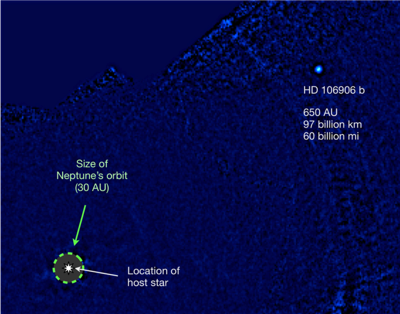
\includegraphics[width=0.6\textwidth]{exoplanet.png}
% \caption{Image of exoplanet HD 106906 b taken with the Magellan Adaptive Optics (MagAO) instrument. \cite{bailey2013hd}}
% \label{fig:exoplanet}
% \end{center}
% \end{figure}


Our ability to study exoplanets is limited by the \jrmcom{define more, planet star flux ratio is faint, etc,} high contrast problem. In direct imaging we are detecting the \jrmcom{it's almost never a combo -- it's one or the other}combination of the exoplanet’s \jrmcom{it's not b.b. in any real case, just thermal emission is all you shoudl say} \jrmrmv{blackbody} thermal emission, and the \jrmadd{starlight} reflected \jrmrmv{starlight} off \jrmrmv{of} the exoplanet’s atmosphere\cite{seager2010exoplanets} which is dwarfed by that of the host star. For example, the contrast between the Sun and the Earth is on order $10^{-10}$ in the visible spectrum \jrmcom{also give what it is at 10 um since you intro-ed thermal}. \jrmcom{What are you trying to say here?  It's true by definition in teh previous sentence -- so what point?} This extreme contrast ratio is the same for Earth-sized exoplanets in the habitable zone, and improves to $10^{-8}$ contrast for exoplanets around M-dwarf stars.\cite{males2014direct} \jrmcom{$\leftarrow$ citatons should be inside the period every time} Ground based observatories face additional challenges from aberrations caused by atmospheric turbulence that degrades the resolution of the image and the exoplanet can no longer be resolved \jrmcom{resolved? or does it make the detection more challenging?}.

 Overcoming this contrast problem requires a two-fold solution. The starlight needs to be suppressed by a coronagraph, and the resulting high contrast region called the dark hole needs to be maintained over the course of the observation through extreme adaptive optics (ExA0)  and wavefront sensing and control (WS$\&$C) techniques. ExAO systems operate by propagating light from a guide star to a wavefront sensor, which measures the phase error of the starlight wavefront. A computer then sends commands to shape a deformable mirror (DM) to correct for the phase error, forming a closed feedback loop that compensates for most of the atmospheric distortion. The corrected beam is then passed to a coronagraph which blocks the light from the on-axis star and allows us to detect faint off-axis companions. There are many types of coronagraphs currently used in high contrast imaging; most work by blocking out light using masks and stops\cite{soummer2004apodized}, or using interferometric techniques to destructively interfere light at the focal plane.\cite{foo2005optical} Uncorrected phase errors and  non-common path errors from the ExAO system result in speckles in the focal plane that \jrmcom{better more sciencey sounding work please:} kill coronagraph contrast. These speckles evolve with time\cite{goebel2016evolutionary} so further methods of WF$\&$C in addition to the ExAO closed loop is needed to null speckles \jrmadd{$\leftarrow$ correct, but relevant to this paper?}.  

% GET RID OF DESCRIPTIONS START LISTING, CURRENT TESTBEDS INCLUDE...
The next generation of giant ground and space telescopes \jrmadd{will} have the capability to directly image potentially habitable Earth-like exoplanets for the first time. The ground based Giant Segmented Mirror Telescopes (GSMTs) include\jrmrmv{s} the Thirty Meter Telescope (TMT) \cite{chisholm2020thirty}, the Giant Magellan Telescope (GMT) \cite{fanson2020overview}, and the European Extremely Large Telescope (E-ELT)\cite{ramsay2020eso}. Proposed giant space telescope missions are the LUVIOR and HabEx missions \jrmcom{citations needed}. \jrmadd{Various} jrmrmv{Test-bed}jrmadd{Testbed}s \jrmrmv{in the United States and abroad} are advancing \jrmrmv{path-finding} technology and techniques to enable exoplanet \jrmrmv{research} \jrmadd{imaging} on \jrmrmv{giant telescopes} \jrmadd{the GSMTs}. \jrmcom{How is coronagraphy relevant?  This ought to be in intro of dissertation overall, but not in this paper} \jrmrmv{One area of research is the development of different coronagraphs for telescopes that have complex apertures. There are also test-beds focused on advancing ExAO and WF$\&$C. This included techniques such as Linear Dark Field Control (LDF), Electric Field Conjugation (EFC), and Low Order Wavefront Sensing (LOWFS).} Current testbeds include the High Contrast Imager for Complex Aperture Telescopes (HiCAT)\cite{2014SPIE.9143E..27N} at the Space Telescope Science Institute, the High-Contrast High-Resolution Spectroscopy for Segmented Telescopes (HCST)\cite{jovanovic2018high} test-bed at the California Institute of Technology, the Decadal Survey Testbed\cite{belikov2014ames} at the NASA Jet Propulsion Laboratory (JPL), the LAM-ONERA On-sky Pyramid Sensor test-bed (LOOPs) (CITE) at the Laboratoire d'Astrophysique de Marseille, the Occulting Mask Coronagraph\cite{shi2017dynamic} test-bed also at JPL, and the High Contrast High- Resolution Spectroscopy for Segmented telescopes Testbed (HCST) (CITE) at the California Institute of Technology. The Magellan Extreme Adaptive Optics system (MagAO-X)\cite{males2020magao} developed \jrmrmv{by the University of Arizona Extreme Wavefront Control Lab (XWCL)} for the Magellan Clay Telescope, doubles as an \jrmrmv{extreme adaptive optics} \jrmadd{ExAO} test-bed. Predictive real time control algorithms are being explored on MagAO-X to improve ExAO correction.\cite{haffert2021data} \jrmrmv{The} MagAO-X \jrmrmv{instrument} \jrmrmv{has also been involved with testing LDFC}\jrmcom{no LDFC has been peformed on MagAO-X!}\jrmrmv{, and using} \jrmadd{employs} a Vector Apodizing Phase Plate Coronagraph (vAPP)\cite{snik2012vector} to enable low order modal wavefront sensing.\cite{2019JATIS...5d9004M} \jrmcom{you should mention and cite SCExAO, just enough to say that MagAO-X is similar to SCExAO} There are many more high-contrast imaging testbeds in existence, and many are listed on the Community of Adaptive OpTics and hIgh Contrast testbeds website.(CITE) A recent summary of current coronagraphy test-beds for space missions can be found in the decadal white paper.\cite{mazoyer2019high}

\jrmrmv{The Extreme Wavefront Control Lab has developed t} \jrmadd{T}he Comprehensive Adaptive Optics and Coronagraph Test Instrument (CACTI) \jrmrmv{for further experimentation in ExAO, WF$\&$C, and coronagraphy. The CACTI test-bench} was designed with the flexibility to support visiting instruments and to be easily re-configurable to perform multiple experiments. \jrmcom{test-bench sounds very colloquial to me.  I only ever hear UA OSC grad students say it.  And I don't think papers should refer to themselves:} \jrmrmv{In this paper} \jrmadd{Here} we describe the design of \jrmrmv{the} CACTI \jrmrmv{test-bench} and \jrmrmv{the current laboratory} \jrmadd{its current} status. We then discuss an experiment performed on CACTI with a visiting three-sided pyramid wavefront sensor (3PWFS) to explore an alternative wavefront sensor architecture for GSMT-ExAO. The pyramid wavefront sensor (PWFS) acts like a Foucault test in two dimensions. Light from the telescope is focused onto a glass pyramid tip where it is split and then the pupil plane is re-imaged onto a detector. The result is copies of the telescope pupil that contain intensity fluctuations that are related to the wavefront phase. All current PWFS on telescopes use a four sided pyramid (4PWFS), resulting in four pupil \jrmrmv{copies} \jrmadd{images}. The sampling of each of the pupils sets the number of modes the ExAO system can correct \jrmrmv{for}. ExAO systems \jrmrmv{need} \jrmadd{require} high sampling of wavefront\jrmadd{s} to optimize performance and as a result require large\jrmrmv{r} detectors. Detector size, speed, and noise all impose limits on wavefront sensor performance. The 3PWFS is less sensitive to read noise than the 4PWFS because \jrmrmv{the 3PWFS creates only three copies of the pupil and as a result} \jrmadd{it} uses \jrmrmv{less}\jrmadd{FEWER FEWER FEWER FEWER FFEWERWERWERWE1!!!!!!!} detector pixels. The 3PWFS has further benefits; a high quality three-sided pyramid optic is easier to manufacture than a four-sided pyramid. Schatz et al. (CITE) determined in simulation that the 3PWFS meets and can exceed the performance of a 4PWFS for a detector with high read noise. \jrmrmv{To continue this research we integrated a real} \jrmadd{Both a} 3PWFS and 4PWFS \jrmadd{were integrated into} \jrmrmv{on} \jrmrmv{the} CACTI \jrmrmv{test-bench} to \jrmadd{demonstrate the operation of a 3PWFS and compare it to the 4PWFS.} \jrmrmv{test the performance of each PWFS at different levels of turbulence.}

\section{Design of \jrmrmv{the} CACTI \jrmrmv{Test-bench} \jrmcom{say Testbed if you must have something here}}
\jrmrmv{The} CACTI \jrmrmv{test-bench} was designed to model a full end-to-end adaptive optics system and have the flexibility to support multiple experiments. In the \jrmrmv{current} \jrmcom{it won't be current by the time this is published} configuration \jrmadd{described here} CACTI consist\jrmadd{ed}\jrmrmv{s} of two \jrmrmv{test-beds} \jrmadd{components}, an adaptive optics simulator and a pyramid wavefront sensor \jrmrmv{test-bed} \jrmadd{testbed}. \jrmcom{Maybe don't mention the fig and table here, instead wait until the next section?} The optical design of \jrmrmv{the} CACTI \jrmrmv{test-bed} \jrmrmv{was done in Zemax can be found} \jrmcom{this isn't an advert., don't name vendors unless it's really relevent} \jrmadd{is shown} in Figure \ref{fig:CACTIZemax}\jrmrmv{.} \jrmadd{, and} Table \ref{tab:CACTItable} summarizes \jrmrmv{all of} \jrmcom{summarizes and all are contradictory} the \jrmadd{main} components\jrmrmv{ in CACTI}. In the following sections we describe \jrmadd{ the optical design} in detail\jrmrmv{ the optical design of CACTI}. 

\begin{table}
	\begin{center}
		\begin{tabular}{ | l| l | }
			\hline
			\textbf{Component}& \textbf{Description}\\ \hline
			Light Source & Helium-Neon laser 633-$nm$ $\lambda$\\ \hline
			Spatial filter & 10-$\mu m$ Pinhole \\ \hline
			Off-axis parabolic mirrors & 375.25-mm Focal length, 23$^{\circ}$ off-axis angle \\ \hline
            Entrance pupil & 7.5-mm Clear aperture mask \\ \hline
            Boston Micromachines deformable mirror & 1024 Actuators, 9mm in diameter \\ \hline
            Beamsplitters & 50/50 Cube beamsplitter \\ \hline
            Modulation Mirror &  PI S-331 Piezo-actuator stage \\ \hline
            3PWFS Optic & Fused silica glass monolith \\ \hline
            4PWFS Optic & Crossed roof prisms \\ \hline
            Science Camera (Camsci) & Basler ACE acA640-750um CMOS\\ \hline
            3PWFS Camera (Camzyla) & Zyla 4.2+ sCMOS detector \\ \hline
            4PWFS Camera (Cam4p) & Basler ace acA720-520um CMOS \\ \hline
            Lens 1 (L1) & Doublet 500-mm focal length  \\ \hline
            Lens 2 (L2) & Doublet (CHECK ZEMAX)  \\ \hline
            Lens 3 (L3) & Custom achromatic air-spaced triplet  \\ \hline
            3PWFS Camera lens 1 (C1) & Doublet 30-mm focal length \\ \hline
            3PWFS Camera lens 2 (C2) & Doublet 30-mm focal length \\ \hline
            4PWFS Camera lens 1 (C3) & Doublet 50-mm focal length \\ \hline
            4PWFS Camera lens 2 (C4) & Doublet 30-mm focal length \\ \hline
				
			\end{tabular}
		\end{center}
	\caption{CACTI components}
	\label{tab:CACTItable}
\end{table}

\begin{figure}
    \centering
    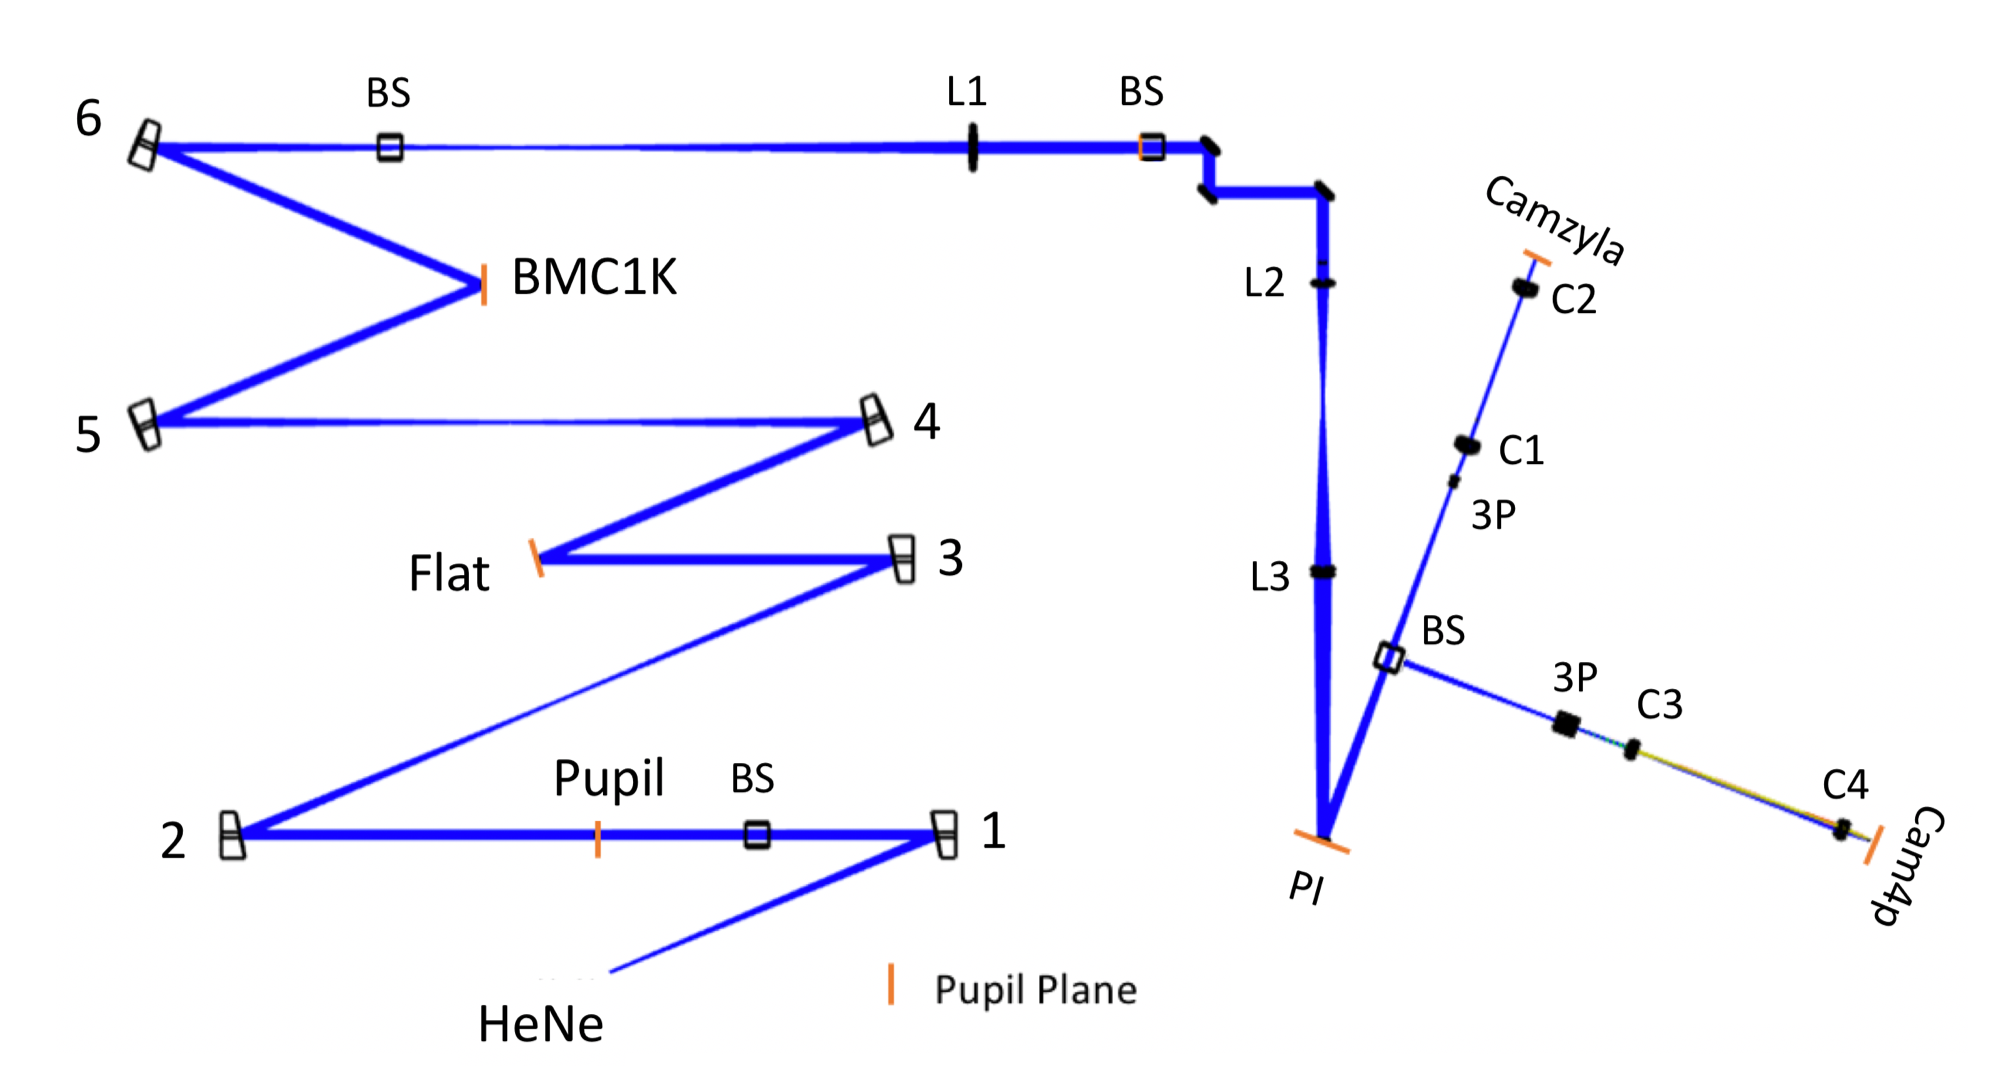
\includegraphics[width=0.8\textwidth]{CACTIzemax.png}
    \caption{IDK if this is good here but it should probably go somewhere}
    \label{fig:CACTIZemax}
\end{figure}

\subsection{Adaptive Optics Simulator}

Adaptive optics (AO) systems operate under the concept of conjugate imaging. Light from the guide star travels through the layers of Earth's atmosphere and acquires phase errors from atmospheric turbulence. In single conjugate AO we model the effects of atmospheric turbulence as a single phase screen at a known altitude that imparts all of the phase errors to the guide star's wavefront. This layer of turbulence is typically modeled to be in the entrance pupil and is imaged to conjugate planes in the AO system. The optical design of an AO system consists primarily of pupil relays that re-size and re-image the pupil plane onto the wavefront sensor and DM so that the turbulence screen is both sensed and corrected in the same plane. Adaptive optics systems work over a wavelength bandpass; to mitigate the effect of chromatic aberrations through the system mirrors are used as the optics in these pupil relays. In a closed loop AO system the wavefront sensor is placed after the DM. When the loop is closed the wavefront sensor sees a wavefront that is the combination of the atmospheric turbulence and the correction applied to the DM. There is a time lag between when the wavefront is sensed and when the correction applied which results in uncorrected wavefront errors that are quantified by the temporal error in the AO error budget. ExAO systems are designed to be low latency and run at loop speeds greater than 1-kHz.

\begin{figure}
    \centering
    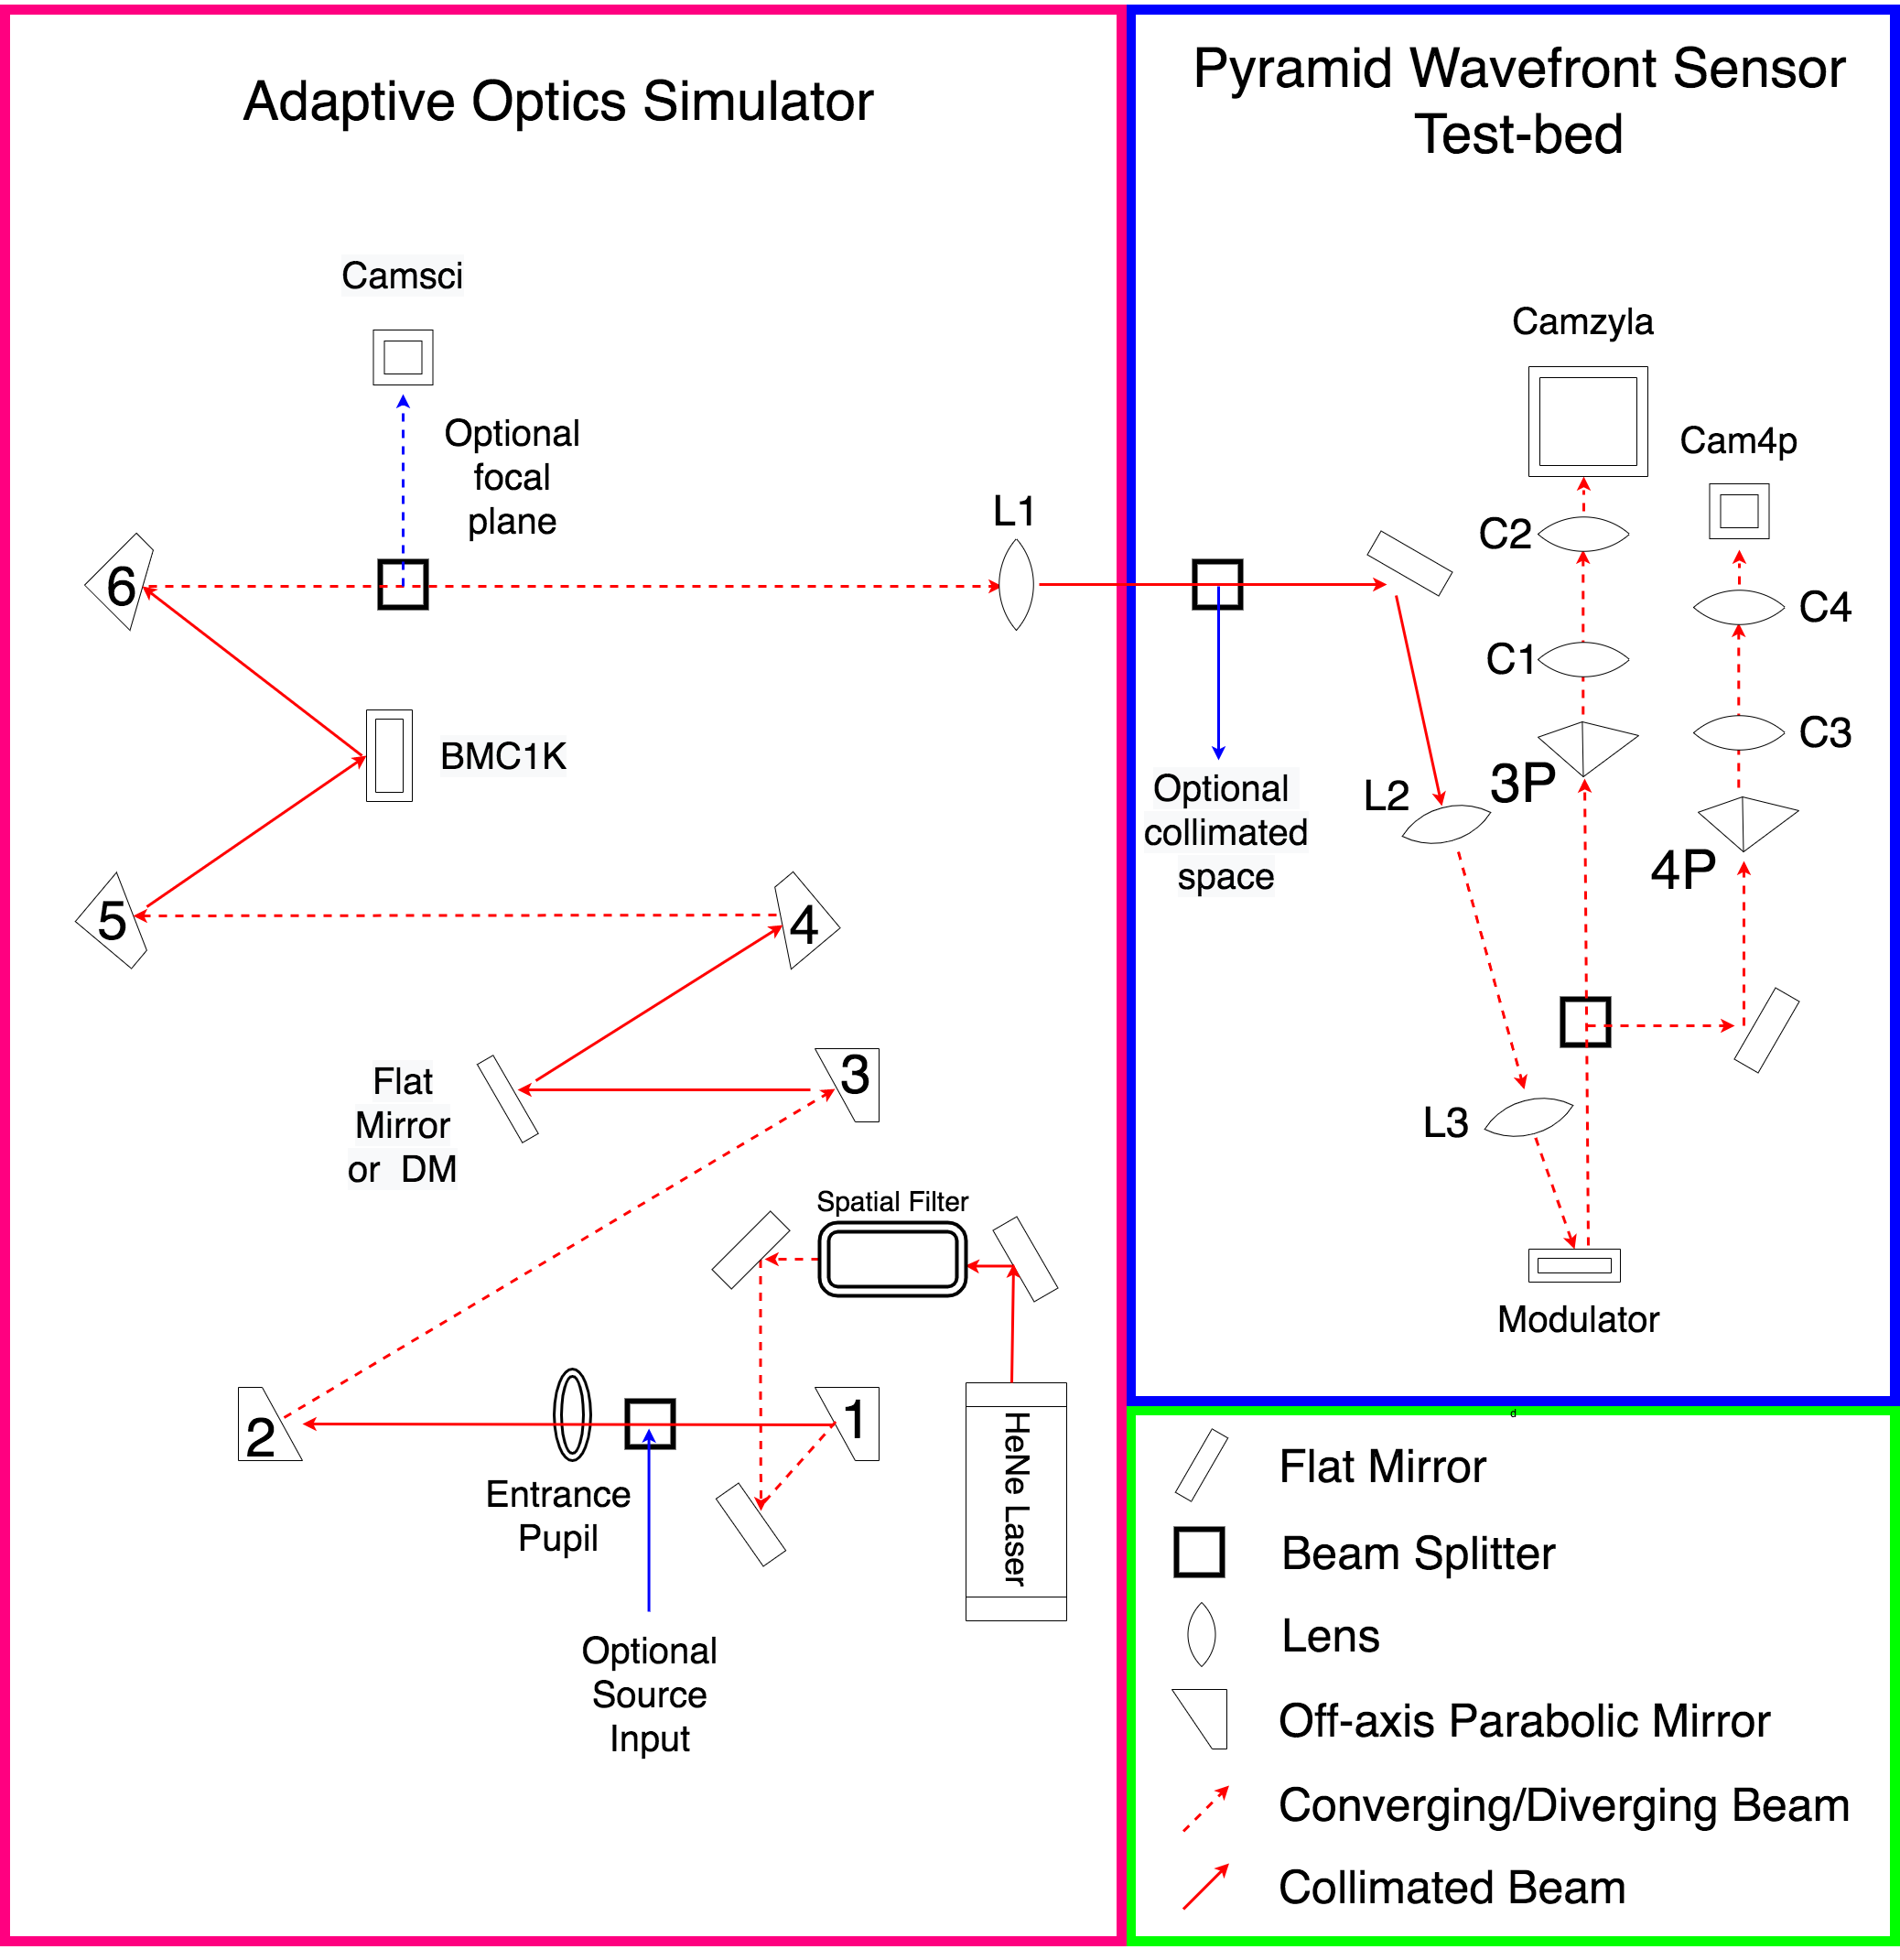
\includegraphics[width=0.8\textwidth]{CACTI.png}
    \caption{Caption}
    \label{fig:CACTI}
\end{figure}

\jrmcom{remove all instances of test-bench.  make it testbed if it is really needed, but try to just say CACTI, and do that fewer times}
\jrmrmv{The} CACTI \jrmrmv{test-bench} was designed to simulate \jrmrmv{realistic} atmospheric turbulence and \jrmrmv{create} a complete closed loop AO system. The layout \jrmrmv{of the CACTI tesbed} is shown in Figure \ref{fig:CACTI}. \jrmrmv{To start the CACTI uses a} \jrmadd{A} Helium-Neon (HeNe) laser \jrmrmv{that has a wavelength of} \jrmadd{(wavelength }633-$nm$\jrmadd{)} \jrmadd{is used for inital alignment and testing}\jrmrmv{as its primary light source}.  The \jrmrmv{laser} \jrmadd{light} is passed to a spatial filter with a 10-$\mu m$ pinhole to clean up any wavefront errors, and insure that the start of the system is an unresolved point source. The point source is then collimated by an off-axis parabolic (OAP) mirror to simulate starlight coming from infinity. \jrmrmv{The CACTI test-bench has} \jrmadd{There are} six OAP mirrors in total that form the pupil relays of the system. All \jrmrmv{6 OAPs} are cored from the same parent with \jrmrmv{an optical surface quality of} $\lambda /10$ \jrmadd{surface quality} \jrmadd{(}Peak-to-Valley\jrmadd{)}. Each OAP has a focal length of 375.25-$mm$ and an off-axis angle of 23 degrees. A 50/50 beamsplitter cube is placed into the collimated beam after the first OAP as an optional input for another collimated light source. After the beamsplitter a 7.5-$mm$ in diameter circular clear aperture mask is placed to define the entrance pupil of CACTI. The first pupil relay formed by the 2$^{nd}$ and 3$^{rd}$ OAP mirrors re-images the entrance pupil onto a flat mirror that is mounted on a kinematic base. The flat mirror is intended to be removed and replaced by a DM \jrmadd{in the future}. \jrmrmv{For a future experiment in segmented aperture mirror phasing for space telescopes we plan to replace the flat mirror with an Iris AO DM that has hexagonal mirror segments that can be actuated in piston, tip and tilt.} The second pupil relay created by the 4$^{th}$ and 5$^{th}$ OAP mirrors, relays the pupil onto \jrmrmv{the permanent DM in the system, which is} a \jrmadd{1024 actuator} Boston Micromachine 1K (BMC1K) DM\jrmrmv{ that has 1024 actuators}. \jrmrmv{We use the DM for the generation of basis set modes,} \jrmadd{In the experiments described here, the BMC1K is used to} to simulate the atmosphere, \jrmrmv{and to} correct the errors \jrmrmv{we apply} in \jrmrmv{a} closed \jrmrmv{feed back} \jrmadd{-}loop with the wavefront sensor\jrmadd{,}\jrmrmv{. The BMC1K was also used to} \jrmadd{and} correct for \jrmadd{common path errors from} misalignment\jrmadd{s}\jrmrmv{ of the optics in the system}. 

\jrmcom{Maybe a software subsection goes here?}

\jrmrmv{The real time control software for the CACTI test-bench is } \jrmadd{CACTI uses} the Compute And Control For Adaptive Optics (CACAO) real-time control software package \cite{guyon2018compute}. The calibration of the AO system by CACAO is a multi-step process. Hadamard modes are applied to the DM, and the WFS response is recorded. The WFS signals from the Hadamard modes are then decomposed into the response of the influence functions from single actuators. These influence functions are then projected onto Fourier modes to create the basis set for the modal wavefront control. In these steps the illumination pattern of the deformable mirror is determined by thresholding actuators that don't give a response in the wavefront sensor. Similarly a mask of the PWFS detector pixels is generated to keep only the valid pixels from the PWFS pupils on the detector that will be used for wavefront sensing. CACAO is also used to generate the phase screens to simulate turbulence. \jrmadd{Due to the limited low-order stroke of the BMC1K,} \jrmrmv{T}\jrmadd{t}he power-spectrum of the turbulence generated by CACAO does not match that of the \jrmcom{this is a subtle thing.  It does match K at higher spatial frequencies, reorganize this} Kolmogorov (CITE) atmospheric turbulence. The power of low order modes of the turbulence are filtered so that the full stroke of the DM is not used. \jrmrmv{The power spectrum of the resulting turbulence is designed to match that of the turbulence corrected by the AO188\cite{clergeon2018subaru} adaptive optics system that is upstream of SCExAO. (IS THAT ACTUALLY TRUE THOUGH?)} \jrmcom{This should be in the previous paragraph, it's not part of r/t control s/w:} The last OAP focuses the light to the final focal plane in the AO simulator. A 50/50 beamsplitter is placed in this converging beam so that an additional focal plane can be accessed. In the current configuration of CACTI we have placed a Basler ACE CMOS camera as our science camera (Camsci) at this focal plane.


\subsection{Pyramid Wavefront Sensor \jrmrmv{Test-bed}\jrmadd{Testbed}}

The pyramid wavefront sensor \jrmrmv{test-bed} \jrmadd{testbed} is a visiting experiment to compare the performance between a 3PWFS and a 4PWFS in varying level of turbulence. \jrmcom{don't you already say all this in the intro? check you organization of this and the intro:} The PWFS operates as a Foucault knife edge test in two dimensions. Light is focused onto the pyramid tip, and the edges of the pyramid divide the focal plane into segments. The apex angle of the pyramid imparts a tilt to each of the segments resulting in spatially separated copies of the pupil on the detector. The diffraction off of the pyramid edges encodes the phase error of the wavefront into the intensity pattern detected in the pupils via a Hilbert transform. CITE (verinaud, myself ;D). The PWFS has four main components, a focusing optic, the pyramid optic, a camera lens, and the detector. The pyramid optic needs to be high quality so that performance is not lost due to manufacturing errors. Common manufacturing errors of pyramid optics include chipping and roofing of the pyramid tip. To mitigate loss of performance a slow beam is focused onto the pyramid tip, so that the spot size is large compared to any potential defects. The size and spacing of the pupil on the detector is set by a combination of the apex angle of the pyramid and the camera lens. The spatial sampling of each of the pupils controls the number of modes the AO system can correct for, and the number of pixels sampling each pupil should be at least equal the number of actuators on the deformable mirror to optimize the AO system. There is a benefit to oversampling the pupils to avoid effects of aliasing at the cost of introducing more read noise. The PWFS is highly sensitive but suffers from a lack of dynamic range. To increase the linearity of the PWFS the PSF on the focal plane of the pyramid tip is modulated in a circle by a piezo-actuated mirror. The effect of modulation is to increase the linearity of the PWFS at the expense of sensitivity. 

ExAO systems need high sampling of the wavefront to optimize performance and as a result require larger detectors. An ideal wavefront sensing camera for ExAO has a large number of pixels that can be read out at a fast speed with low read noise. Current detectors are limited so there is a trade-off between detector, size, speed and performance. We are interested in exploring the 3PWFS as an alternative wavefront sensor for the GSMTs because the 3PWFS uses fewer detector pixels than the 4PWFS. Previous work has shown in simulation that because of this the 3PWFS is less sensitive to read noise, resulting in a modest boost in performance. (CITE myself). On CACTI we want to test the performance of a real 3PWFS, and expand the previous study to understand how the 3PWFS performs under different turbulence conditions compared to the 4PWFS. 

The design of the PWFS test-bed is detailed in Figure \ref{fig:CACTI}. Light from the AO simulator is collimated by a 500-mm focal length lens (L1) which relays the exit pupil of the AO simulator to the PWFS test-bed. The exit pupil of the AO simulator becomes the entrance pupil to the PWFS test-bed, which is then resized by a pupil relay consisting of an achromatic doublet (L2) and a custom air-spaced achromatic triplet lens (L3). The pupil is imaged on the the modulation mirror, which is a $\lambda/20$ flat mirror mounted on a PI S-331 high speed piezo-actuator tip/tilt platform. A 3PWFS designed by Hartsci LLC has been integrated into the instrument for the performance test. The three sided pyramid optic is single prism made from fused silica glass and has a tip smaller than 5 microns that was custom made for this experiment. Figure \ref{fig:pyramidOptics}.A shows the 3D model of the manufactured prism. The 4PWFS in CACTI uses two crossed roof prisms\cite{jovanovic2016scexao} for its pyramid optic shown in Figure \ref{fig:pyramidOptics}.B. This is the same type of pyramid used in the Subaru Coronagraphic Extreme Adaptive Optics instrument (SCExAO)\cite{jovanovic2015subaru}.  A 50/50 beamsplitter after the modulation mirror sends the same PSF to the pyramid tips of the 3PWFS and 4PWFS to mitigate non-common path errors, as all the optics up to that point are common to both wavefront sensors. The PSF on the pyramid tips were sharpened by the DM using an eye-doctor script. The script is a grid search that applies different amplitudes of Zernike modes on the deformable mirror, and saves the combination of modes that maximizes the Strehl Ratio at the focal plane as the  DM set point where non-common path errors are minimized.

\begin{figure}
    \centering
    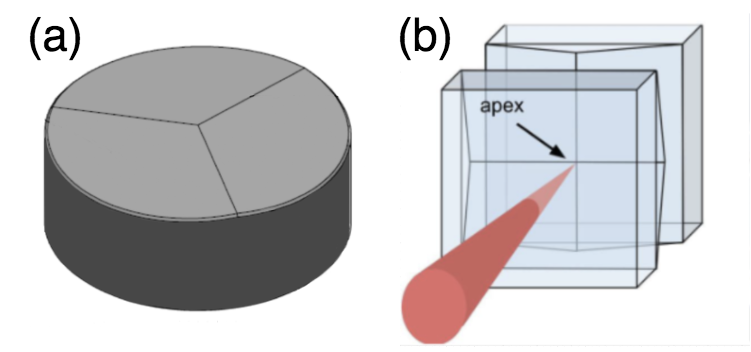
\includegraphics[width=0.8\textwidth]{pyramidOptics.png}
    \caption{4 PWFS Figure 2 in \ref{jovanovic2016scexao}}
    \label{fig:pyramidOptics}
\end{figure}


The pupil of each PWFS are imaged on the the detectors by using two camera lenses, C1 and C2 for the 3PWFS, and C3 and C4 for the 4PWFS,  that form a zoom lens system to insure that the sizes of pupils from both PWFS are 30 pixels in diameter. The 3PWFS uses a Zyla 4.2+ sCMOS detector which has an average read noise of (GO BACK AND FIND). The 4PWFS has a Basler ace acA720-520um CMOS camera that has an average read noise of (GO BACK AND FIND). Schatz et al. found in simulation that when the PWFS are well illuminated by light the effects of read noise to performance are negligible. The experiments performed in this paper were under bright light conditions, so having different cameras with different noise characteristics should not effect the PWFS performance. 

The PWFS signals on CACTI can be processed in two ways, the Raw Intensity (RI) and Slopes Maps (SM) methods. In both methods the detector signal from the PWFS is dark subtracted, and a threshold is applied to mask out any pixels outside of the PWFS pupils. In the RI method the remaining signal is used as-is. The Slopes Maps calculation recombines the PWFS pupils into an estimate of the X and Y slopes of the wavefront slope. The SM equation for the 4PWFS is given in Equation \ref{4PWFSslopes}, and the Equation for the 3PWFS is given in \ref{3PWFSslopes}. In these euqations $S_x, S_y$ are the local wavefront slopes, and $I_1...I_4$ are the intensity values of the pixel corresponding to the same location in each pupil.


\begin{eqnarray}
    S_x=\frac{I_1+I_2-I_3-I_4}{I_1+I_2+I_3+I_4}     \label{4PWFSslopes} \\
    S_y=\frac{I_1-I_2-I_3+I_4}{I_1+I_2+I_3+I_4} \nonumber
\end{eqnarray}

\begin{eqnarray}
    S_x=\frac{\frac{\sqrt{3}}{2}I_2-\frac{\sqrt{3}}{2}I_3}{I_1+I_2+I_3} \label{3PWFSslopes} \\
    S_y=\frac{I_1-\frac{1}{2}I_2-\frac{1}{2}I_3}{I_1+I_2+I_3} \nonumber
\end{eqnarray}

\subsection{Current Status}

The alignment of the CACTI test-bed was completed in May 2020. Figure \ref{fig:cactiTestbed} is a picture of the as built system. Light from the HeNe laser is relayed by the six OAP mirrors, and is then coupled to the PWFS test-bed using a beam triangle formed by two flat mirrors. Figure \ref{fig:PWFStestbed} is a close up diagram of the PWFS test-bed. The first two lenses (L1 and L2) relay the entrance pupil of the PWFS testbed onto the PI modulation mirror (PI). A beamsplitter after the modulation mirror picks off light to the four-sided pyramid (4P) and the through beam is sent to the three-sided pyramid (3P). Both pyramids have two camera lenses (C1 and C2) that form a zoom lens to match the diameters of the pupils of the two PWFS. The measured pupil diameter for the 4PWFS is 30.5 pixels and 29.5 pixels for the 3PWFS. 

\begin{figure}
    \centering
    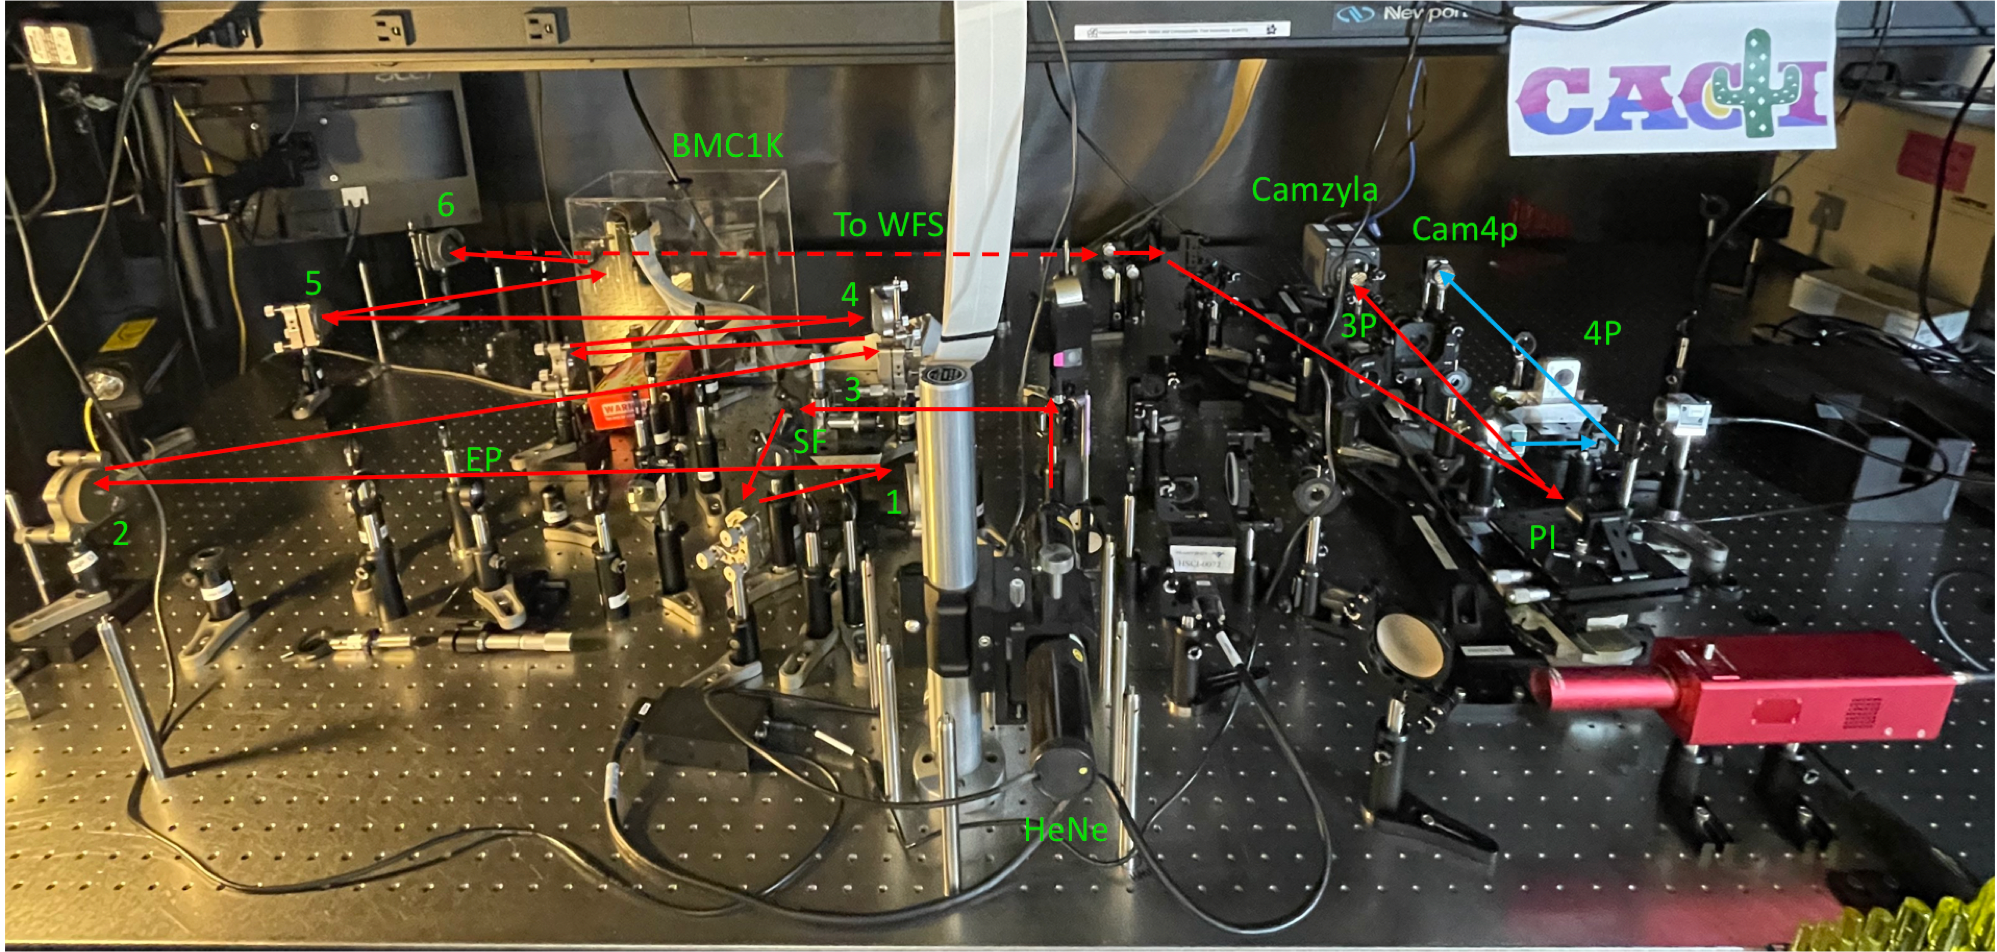
\includegraphics[width=0.8\textwidth]{cactiTestbed.png}
    \caption{Caption}
    \label{fig:cactiTestbed}
\end{figure}

\begin{figure}
    \centering
    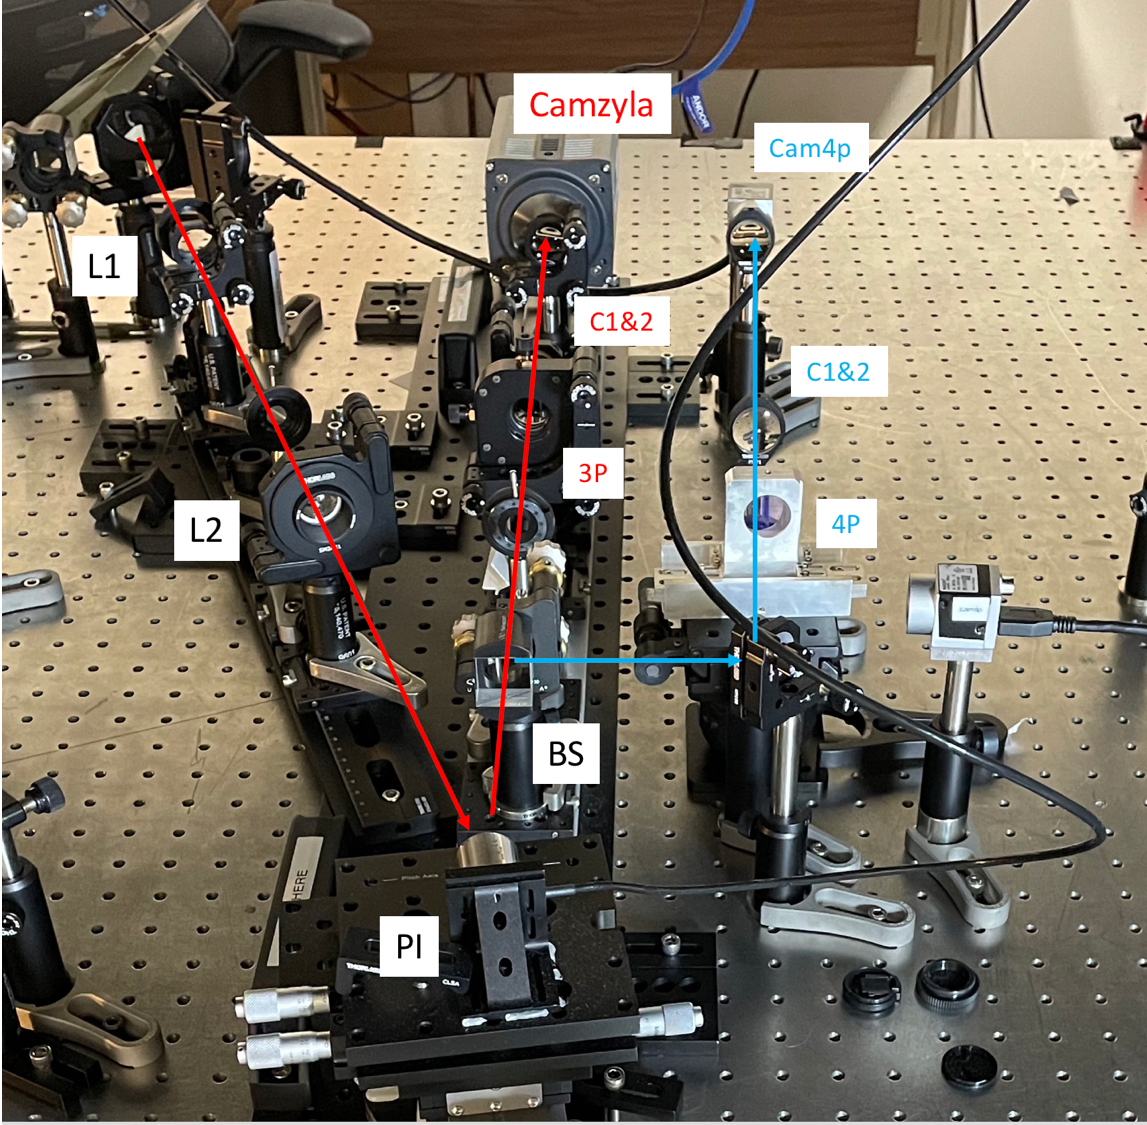
\includegraphics[width=0.8\textwidth]{PWFStestbed.png}
    \caption{Caption}
    \label{fig:PWFStestbed}
\end{figure}


The PSF at the pyramid tip was optimized by an eye-doctor script to generate the flat commands for the deformable mirror. The system responses to the flat wavefront generated by the deformable mirror is given by Figure \ref{fig:flatCACTI}. Figure \ref{fig:flatCACTI}.A is the PSF in logarithmic scale on our science camera. Figure \ref{fig:flatCACTI}.B similarly is the PSF on the pyramid tip also in log scale. Figure  \ref{fig:flatCACTI}.C and Figure \ref{fig:flatCACTI}.D are the pyramid pupils from a flat wavefront with 5$\lambda/D$ modulation for the 3PWFS and 4PWFS respectively. 

\begin{figure}
    \centering
    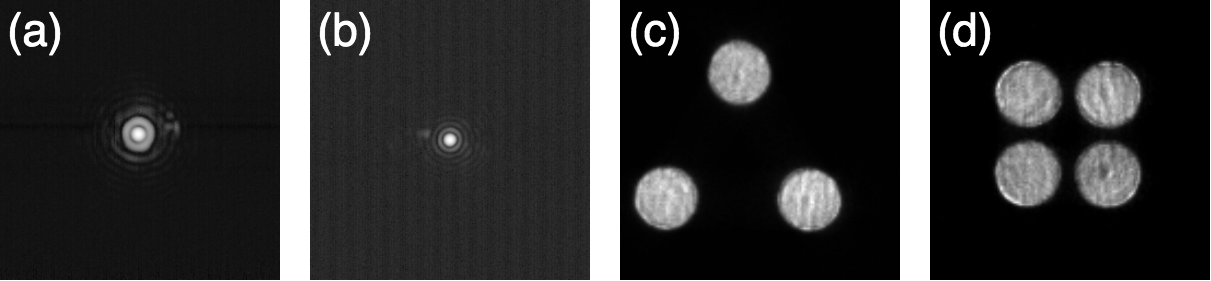
\includegraphics[width=0.8\textwidth]{flatCACTI.png}
    \caption{Caption}
    \label{fig:flatCACTI}
\end{figure}


We have successfully closed the AO loop on the CACTI test-bed with both the 4PWFS and 3PWFS using both the RI and SM signal handling methods. Closing the loop on this 3PWFS is a major milestone for the development of the three-sided pyramid wavefront sensor, because this is the first time the loop has been closed on a 3PWFS built with a real glass pyramid prism. Previous work by Schatz et al. closed the AO loop on a 3PWFS on the LOOPs test-bed at the Laboratoire d'Astrophysique de Marseille. The 3PWFS on the LOOPs test-bed was created by a phase screen applied to a spatial light modulator. The deformable mirror on CACTI was used to both generate the turbulence screen and apply the correction. This is done using the CACAO software which creates multiple channels of commands for the deformable mirror. In one channel we can stream the turbulence phase screens, and in another channel we have the commands computed by real time control software using the PWFS signals. The actual command applied to the DM is a summation of commands from all of the channels. Figure \ref{fig:turbCACTI} shows the closed loop PSFs and pyramid pupils from a turbulence strength of 0.3-$\mu m$ RMS error on CACTI. Figure \ref{fig:turbCACTI}.A and \ref{fig:turbCACTI}.B are the 3PWFS pupils and the closed loop PSF in log scale on the science camera. Figure \ref{fig:turbCACTI}.C and \ref{fig:turbCACTI}.D are the 4PWFS pupils and the closed loop PSF in log scale on the science camera.


\begin{figure}
    \centering
    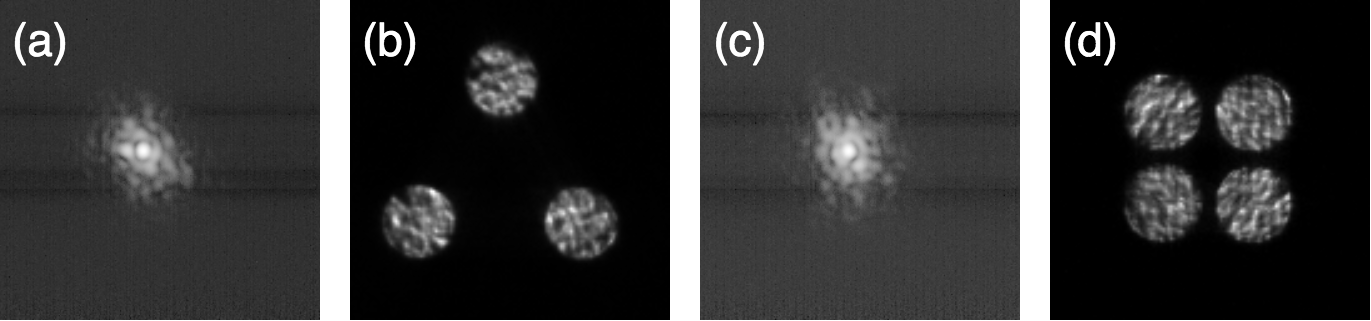
\includegraphics[width=0.8\textwidth]{turbCACTI.png}
    \caption{Caption}
    \label{fig:turbCACTI}
\end{figure}

\begin{table}
	\begin{center}
		\begin{tabular}{ | l|l|l | }
			\hline
			\textbf{Camera}& \textbf{Model} &\textbf{Read Noise}\\ \hline
             Camsci & Basler ACE acA640-750um CMOS  & 12.25 $e^-$ read noise\\ \hline
             Camzyla & Zyla 4.2+ sCMOS detector & 7.98 $e^-$ read noise \\ \hline
             Cam4p & Basler ace acA720-520um CMOS & 0.11 $e^-$ read noise \\ \hline
             Camtip & Basler ACE acA640-750um CMOS (DOUBLE CHECK)  & 9.30 $e^-$ read noise\\ \hline
				
			\end{tabular}
		\end{center}
	\caption{CACTI components}
	\label{tab:CACTItable}
\end{table}


\section{Experimental Details}

The CACTI testbed was used to compare the performance of a 3PWFS and 4PWFS in varying strengths of turbulence. Previous work by Schatz et al. found in simulation that the performance of the two wavefront sensors are comparable. These simulations however were run for only one seeing condition. The goal of this experiment is to determine the relative performance of the 3PWFS to the 4PWFS in varying strengths of turbulence using both the Raw Intensity and Slope Maps signal processing methods. The performance was determined by measuring the relative Strehl ratio of the AO corrected PSF and the aberration free PSF. For the CACTI testbed our aberration free PSF was the flat wavefront PSF on the science camera created by the deformable mirror shown in Figure \ref{fig:flatCACTI}.A., which we will refer to as the reference PSF. To calculate the Strehl Ratio we developed a Strehl Calculation pipeline detailed in Appendix A. The Strehl ratio is calculated by taking the ratio of the peak intensity of the partially corrected PSF, $P_{data}$,  to the peak intensity of the reference PSF, $P_0$. The peaks are normalized by the flux in the image. 

\begin{equation}
    S=\frac{P_{data}/Flux_{data}}{P_{0}/Flux_{0}}
    \label{Strehl}
\end{equation}

The first experiment performed on CACTI was to measure the Strehl Ratio as a function of turbulence strength and modulation radius for both the 3PWFS and the 4PWFS.  This experiment was performed using the Raw Intensity signal handling method. The modulation radii used were: 1.6 $\lambda/D$, 3.25 $\lambda/D$, and 5 $\lambda/D$. At each modulation radius the following experiment was performed. For all experiments the loop speed was 400-Hz.

\begin{itemize}
    \item Apply the best flat commands on the DM and create the reference PSF from the average of 1000 frames
    \item Dark frames taken for each of the cameras. Dark frames created from an average of 1000 frames
    \item A new calibration and reconstructor matrix was taken for each modulation radius.
    \item Apply simulated turbulence at levels 0.1-$\mu m$, 0.2-$\mu m$, 0.3-$\mu m$, 0.4-$\mu m$, 0.5-$\mu m$ RMS wavefront error. 
    \item At each level of turbulence strength, generate 5 different phase screens
    \item At each phase screen record 50 closed-loop PSF images, where each image is created from taking the average from 200 frames of data. 
    \item Calculate the average Strehl value from the closed-loop PSFs and average the Strehl ratio over the 5 trails to create an average Strehl value for each turbulence strength.
    \item Plot the Strehl value as a function of turbulence strength and magnitude radius. 
    
\end{itemize}





	
 


%An adaptive optics system works on the concept of conjugate imaging. An object plane corresponding to a layer of atmospheric turbulence is imaged through the telescope AO system onto a deformable mirror where the correction is applied. To achieve this the bulk of an AO system on sky or in the lab consists of pupil relays.

% \begin{figure}
%     \centering
%     \includegraphics[width=1\textwidth]{psfs.png}
%     \caption{PSFs on the science camera with A) Flat Wavefront, B) Turbulence, C) AO Corrected Turbulence.}
%     \label{fig:PSF}
% \end{figure}

 

% \begin{figure}
%     \centering
%     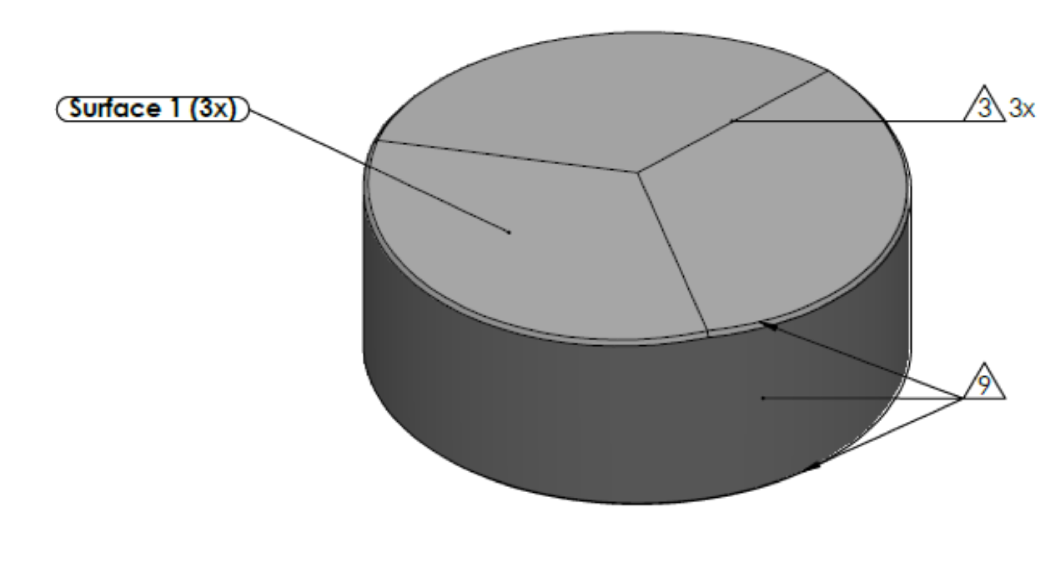
\includegraphics[width=0.5\textwidth]{3poptic.png}
%     \caption{The 3D model of the refractive 3 side pyramid optic.}
%     \label{fig:3poptic}
% \end{figure}




\section{Results}

\begin{figure}
    \centering
    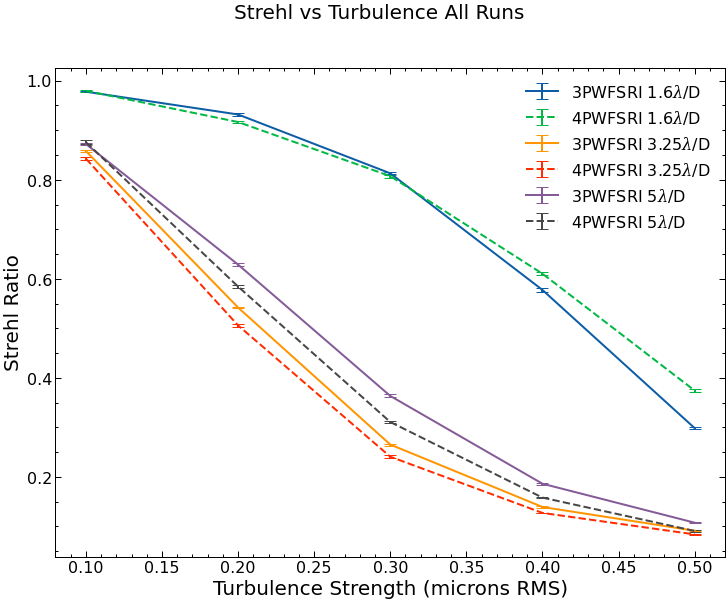
\includegraphics[width=0.8\textwidth]{StrehlvsTurbRI4vs3.png}
    \caption{Caption}
    \label{fig:my_label}
\end{figure}
\section{Discussion}
\section{Conclusion}

\appendix
\section{Strehl Ratio Calculation}

An adaptive optics system compensates phase errors to return the resolution of the system to the diffraction limit of the telescope. The correction is not perfect, and we are interested in measuring the performance of the AO system. The Strehl ratio relates the residual uncorrected phase errors to the AO corrected PSF. The Strehl ratio is defined as,

\begin{equation}
    S \cong e^{-\sigma^2}
\end{equation}

where $S$ is the Strehl ratio, and $\sigma^2$ is the residual RMS phase error. The measurement of the Strehl ratio for an AO corrected PSF is given in Equation \ref{Strehl}. The Strehl ratio is calculated by taking the ratio of the peak intensity of the partially corrected PSF, $P_{data}$,  to the peak intensity of an aberration free PSF, $P_0$. The peaks are normalized by the flux in the image. A simulated model can be used for the aberration free image. 

\begin{equation}
    S=\frac{P_{data}/Flux_{data}}{P_{0}/Flux_{0}}
    \label{Strehl}
\end{equation}

The calculation of Strehl for the data taken from the CACTI testbed was done using a Strehl Ratio Calculation tool that developed in Python. The flow of the Strehl Ratio code is given in Figure \ref{StrehlClass}. The user inputs a list of filenames containing the image files (pathToData) and the image file for the aberration free PSF (pathToPerfect). For the CACTI testbed our aberration free PSF was the flat wavefront PSF on the science camera created by the deformable mirror, which we will refer to as the reference PSF. A simulated perfect PSF matching the plate scale of the system is an alternative. These two paths are the only mandatory inputs to the pipleline. If only one filename is given in pathToPerfect, then that reference PSF will be used in the Strehl calculation for every data file. If multiple files are used for the reference PSF, than the number of filenames for pathToPerfect must match that of pathToData. In this case, the reference PSF will be used with the data PSF from the filename with the same list index to calculate Strehl. An optional file to read in is pathToDarks which contains the dark files that will be used in dark subtraction. For CACTI the same camera is used to record the AO corrected PSFs and the reference PSF so the dark file is the same and used for both data sets. The pipleline checks that none of the data is saturated, by comparing the max of every image to the hard coded over-saturation value of the science camera which is a value 1023. If any of the data is over-saturated the pipeline with produce an error.

The Strehl ratio is calculated using the peak of the data. The Strehl Calculation Tool can find the peak of each image two different ways. The default method assumes that the highest value in each image is the peak of the data. An optional way is to use the Smart Peak Finder, which is an optional attribute provided by the user. The Smart Peak Finder uses the DAOStarFinder from Astropy that uses a Gaussian fitter to find the peak of the image. The user can provide the full-width half-max (FWHM) of the Gaussian kernel used by DAOStarFinder as an optional object attribute. If the user does not specify a FWHM, the Strehl Calculation tool will estimate the FWHM by pulling a sample image from the referencePSF data, and fitting a Gaussian to the a slice of the PSF created by taking the radial average around the max value in the frame. Once the peak value in each frame is found, the coordinates of that peak are saved for later use in the pipeline. 

The dark subtraction is performed in two steps. First if the user provided a dark files, they are subtracted off of frame. A second round of dark subtraction is done by masking out the PSF, and row by row taking the average value of the row, and subtracting it from that row. The mask is a circular mask centered on the coordinates of the peak found in the previous step. There is a default diameter to the mask which is one third the size of the smallest dimension of the images. A diameter can be provided as an optional input by the user. After dark subtraction the peak value is then pulled from every frame to be used in the Strehl calculation detailed in Equation \ref{Strehl}. The peak is normalized by the Flux in the image. To do this the Strehl Calculation tool sums the Flux in circles of increasing radii that are centered on the peak of the image. The result is a Strehl as a function of radius from the peak. Figure \ref{fig:StrehlVsRadiiExample} is a plot of the output from the Strehl Calculator tool, for a data set of closed loop PSFs from five different files, each file representing a single closed loop run. The turbulence strength for this data set was 0.3 microns RMS. As the radii of the summed Flux increases, the Strehl ratio flattens out which indicates a good background subtraction was done. If the background subtraction was poor, the Strehl ratio would increase as radius increased. Making the diameter of the PSF mask used for background subtraction smaller can help solve this issue. 

\begin{figure}
    \centering
    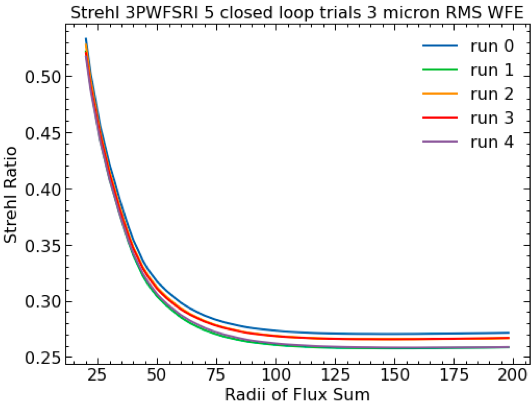
\includegraphics[width=0.8\textwidth]{StrehlVsRadiiExample.png}
    \caption{Caption}
    \label{fig:StrehlVsRadiiExample}
\end{figure}





\begin{figure}
    \centering
    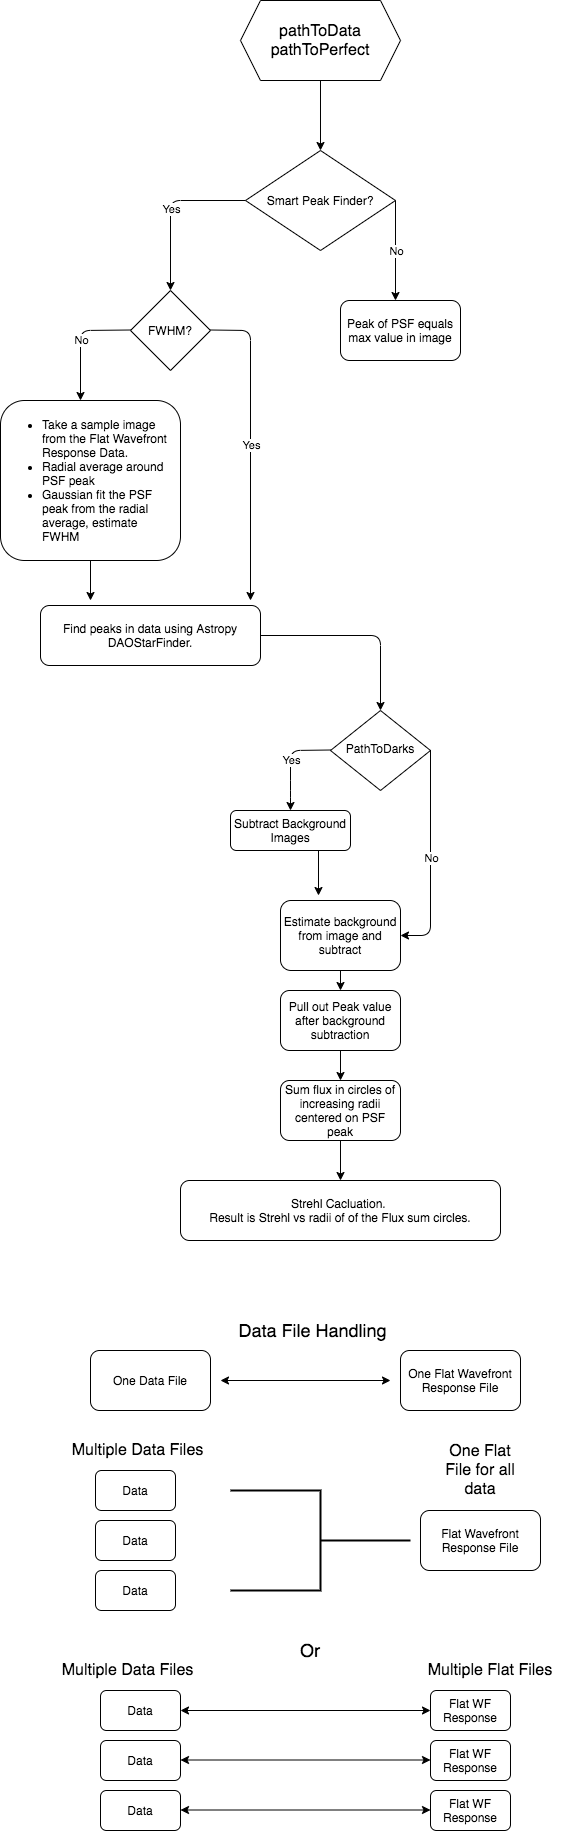
\includegraphics[width=0.8\textwidth]{strehlclass2.png}
    \caption{Caption}
    \label{fig:strehlClass}
\end{figure}

 


%%%%% References %%%%%

\bibliography{report}   % bibliography data in report.bib
\bibliographystyle{spiejour}   % makes bibtex use spiejour.bst

%%%%% Biographies of authors %%%%%

% \vspace{2ex}\noindent\textbf{First Author} is an assistant professor at the University of Optical Engineering. He received his BS and MS degrees in physics from the University of Optics in 1985 and 1987, respectively, and his PhD degree in optics from the Institute of Technology in 1991.  He is the author of more than 50 journal papers and has written three book chapters. His current research interests include optical interconnects, holography, and optoelectronic systems. He is a member of SPIE.

% \vspace{1ex}
% \noindent Biographies and photographs of the other authors are not available.

\listoffigures
\listoftables

\end{spacing}
\end{document}
